\section{Auswertung}
\label{sec:Auswertung}

Aus den gegebenen Prismawinkeln ergeben sich die in Tabelle \ref{tab:1} aufgeführte Dopplerwinkel.

\begin{table}
    \centering
    \caption{Prismawinkel und Dopplerwinkel.}
    \label{tab:1}

    \begin{tabular}{c | c| c| c}
        \toprule
        Prismawinkel & 15$^{\circ}$    & 30$^{\circ}$    & 60$^{\circ}$   \\
        \midrule
        Dopplerwinkel& 80,06$^{\circ}$ & 70,57$^{\circ}$ & 54,74$^{\circ}$\\
        \bottomrule
    \end{tabular}

\end{table}

Mit Gleichung \eqref{equ:Geschw} werden die Geschwindigkeiten der Glaskugeln der Dopplerphantomflüssigkeit bestimmt.
Die berechneten Geschwindigkeiten hängen jeweils von der Frequenzverschiebung und dem Dopplerwinkel ab und 
sind in Tabelle \ref{tab:Geschw} dargestellt.

\begin{equation}
    \label{equ:Geschw}
    v = \frac{\increment \nu \cdot c}{2\nu \cdot cos(\alpha)}
\end{equation}

\begin{table}
    \centering
    \caption{Berechnete Strömungsgeschwindigkeiten.}
    \label{tab:Geschw}

    \begin{tabular}{c | c c c c c c}
        \toprule
        Flussgeschwindigkeit:& 1,5 & 2,5 & 3,5 & 4,5 & 5,5 & 6,5 \\ 
        \midrule
        Rohrinnendurchmesser [mm]   & \multicolumn{6}{c}{Strömungsgeschwindigkeit [$\frac{m}{s}$]} \\
        / Prismawinkel & & & & & & \\
        \midrule
        7 / 15  & 0,222 & 0,415 & 0,897 & 0,892 & 1,210 & 1,528 \\
        7 / 30  &-0,181 &-0,380 &-0,594 &-0,891 &-1,222 &-1,505 \\
        7 / 60  & 0,181 & 0,419 & 0,704 & 1,027 & 1,476 & 1,770 \\
        10 / 15 & 0,128 & 0,159 & 0,255 & 0,381 & 0,508 & /     \\
        10 / 30 &-0,083 &-0,133 &-0,198 &-0,330 &-0,463 & /     \\
        10 / 60 & 0,086 & 0,171 & 0,285 & 0,409 & 0,419 & /     \\
        16 / 15 &  /    & 0,128 & 0,159 & 0,222 & 0,318 & 0,349 \\
        16 / 30 &  /    &-0,083 &-0,115 &-0,198 &-0,281 &-0,364 \\
        16 / 60 & 0,048 & 0,076 & 0,124 & 0,181 & 0,257 & 0,333 \\
        \bottomrule
    \end{tabular}
\end{table}

Graphik \ref{fig:KeineAhnung} zeigt $\frac{\increment \nu}{cos(\alpha)}$ in Abhängigkeit von der Strömungsgeschwindigkeit, für den Dopplerwinkel 
$\alpha = 80,06^{\circ}$ und alle drei Rohre.
Zur Bestimmung der Punkte wird Gleichung \eqref{equ:Geschw} zu 
\begin{equation}
    \frac{\increment \nu}{cos(\alpha)} = \frac{2\nu \cdot v}{c},
\end{equation}
umgestellt.

\begin{figure}
    \centering
    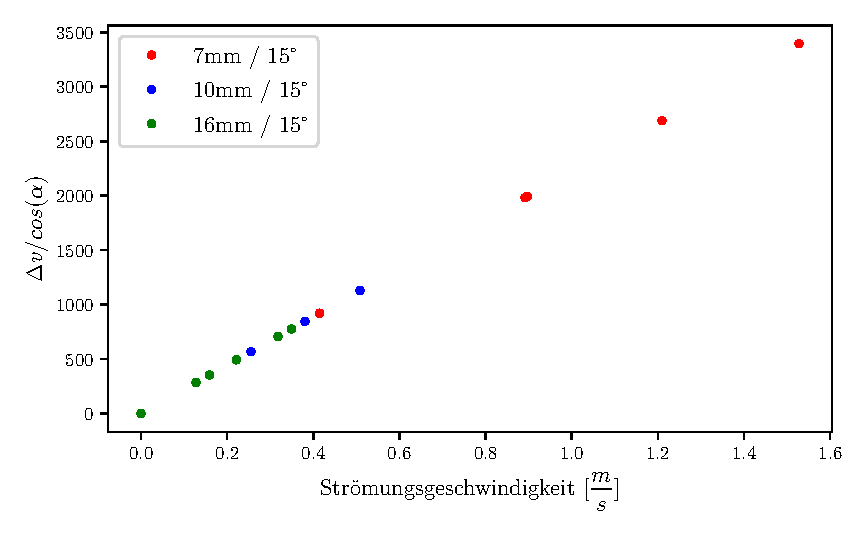
\includegraphics[width = 0.70\textwidth]{plot1.pdf}
    \caption{Verhältnis der Frequenzverschiebung zum Dopplerwinkel abhängig von der Strömungsgeschwindigkeit.}
    \label{fig:KeineAhnung}
\end{figure}

Für das Strömungsprofil werden zunächst die Strömungsgeschwindigkeiten der verschiedenen Tiefen bei einer Pumpleistung von 
70\% bzw. 45\% bestimmt. 
Um das Strömungsprofil veranschaulichen zu können, werden die Strömungsgeschwindigkeiten $v$ berechneten und zusammen mit den Streuintensitäten $I$
in Abhängigkeit von der Messtiefe, in ein Diagramm eingezeichnet. Dies zeigt Graphik \ref{fig:70P} für die 70\% Pumpleistung und Graphik \ref{fig:45P} 
für die 45\% Pumpleistung.

\begin{figure}
    \centering
    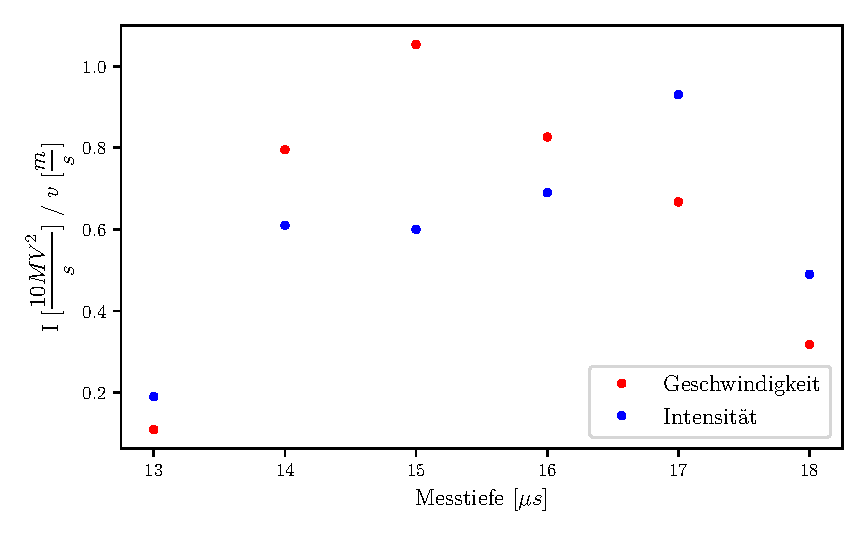
\includegraphics[width = 0.70\textwidth]{plot2.pdf}
    \caption{Strömungsprofil bei 70\% Pumpleistung.}
    \label{fig:70P}
\end{figure}

\begin{figure}
    \centering
    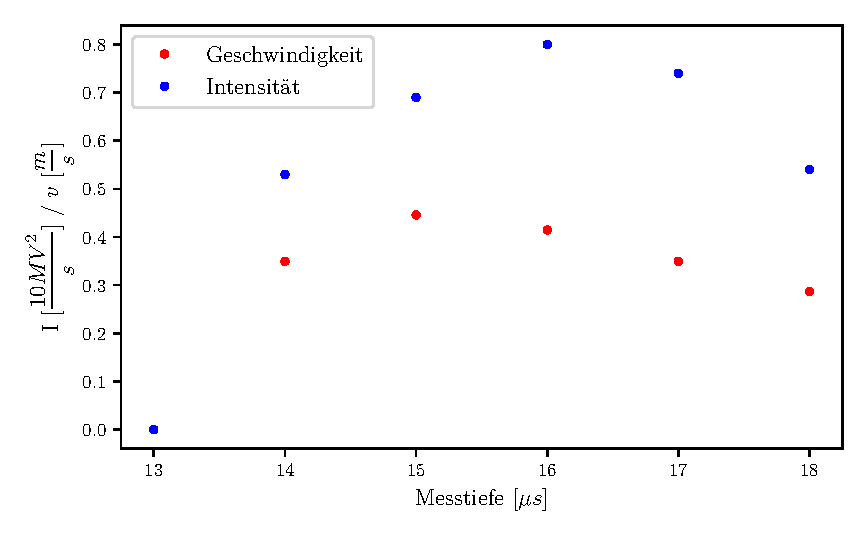
\includegraphics[width = 0.70\textwidth]{plot3.pdf}
    \caption{Strömungsprofil bei 45\% Pumpleistung.}
    \label{fig:45P}
\end{figure}
